
\begin{itemize}

\item[1.] Let $X$ be an $n$-dimensional vector space over $K$. We will denote the \textit{dual} of $X$ by
the set 
$$X' := \{l:X \rar K \ | \ l \text{ is linear}\},$$
and use \textit{scalar product} notation $(l, x) := l(x)$. The transpose of a linear map
$A: X \rar X$ is a linear map $A': X' \rar X'$ defined by $A':l \mapsto m$, where $A(l(x)) = m(x)$ for all $x \in X$.
\begin{enumerate}[(a)]
\item Write out the definition of the transpose map using scalar product
notation, without using ``$m$".
\begin{proof}

\end{proof}

\item Suppose that $A$ has distinct eigenvalues $\lambda_1, . . . , \lambda_n$. Prove that the
corresponding eigenvectors $v_1, . . . , v_n$ are linearly independent.
\begin{proof}

\end{proof}

\item Still using the assumptions of Part (b) let $l_1, . . . , l_n \in X'$ be the \textit{dual basis}, which means that
\begin{equation*}
(l_i, v_i) = \delta_{i,j} =  \left\{
        \begin{array}{ll}
            1 & i=j \\
            0 & i \neq j 
        \end{array}
    \right.
\end{equation*}
Prove that $l_1, . . . , l_n$ are eigenvectors of the transpose map $A': X' \rar X'$.
\begin{proof}

\end{proof}

\item Now, suppose that $f_1, . . . , f_n$ is any basis of eigenvectors of $A'$ corresponding to $\lambda_1, . . . , \lambda_n$. Prove that $(f_i, v_j ) = 0$ if $i \neq j$ and $(f_i, v_i) \neq 0$.
\begin{proof}

\end{proof}

\item For any $x = a_1v_1 + ... + a_nv_n$, derive a formula for $a_i$ in terms of $x$, $v_i$, and $f_i$.
\begin{proof}

\end{proof}
\end{enumerate}








\item[2.] Let $R$ be an arbitrary commutative ring that contains a field $\bbf$ where the multiplicative identity 1 of $\bbf$ is also the multiplicative identity of $R$. For any $a \in R$, define a map $m_a : R \rar R$ via multiplication, that is, $m_a(v) = a \cdot v$ for $v \in R$.
Note that $R$ is a vector space over $\bbf$ and $m_a$ is a linear map on $R$ over $\bbf$. 
An element $\lambda \in \bbf$ is called an eigenvalue for $a$ (or $m_a$) if $av = \lambda v$ for some nonzero
$v \in R$, and such a $v$ is called an eigenvector of $m_a$.
\begin{enumerate}[(a)]
\item Show that $m_a$ is injective (one-to-one) if and only if a is a nonzero
divisor in $R$ (i.e., $ab \neq 0$ for every nonzero $b \in R$). Give an example of $R$ and
$a \in R$ so that $m_a$ is injective but not surjective.
\begin{proof}

\end{proof}

\item Show that $m_a$ is bijective if and only if $a$ is invertible in $R$ (i.e., there
exists $b \in R$ so that $ab = 1$).
\begin{proof}

\end{proof}

\item Suppose $R$ has dimension $n$ as a vector space over $\bbf$. Show that, for
every $a \in R$, there is a monic polynomial $f(y) \in \bbf[y]$ of degree $\leq n$ so that
$f(a) = 0$. (\textbf{Hint}: Fix a basis for $R$ over $\bbf$ and consider the characteristic
polynomial of the linear map $m_a$.)
\begin{proof}

\end{proof}

\item Consider the ring $R = \bbq[x]/(\phi(x))$ where $\phi(x) = x^3-x = x(x-1)(x+1)$. Find all eigenvalues and eigenvectors of $m_a$ for $a = 1 + 2x \in R$. Verify
that you can pick your eigenvectors $v_1, v_2, v_3 \in R$ so that
\begin{equation*}
v_i (p_j) = \delta_{i,j} =  \left\{
        \begin{array}{ll}
            1 & i=j \\
            0 & i \neq j 
        \end{array}
    \right.
\end{equation*}
where $p_1 = -1$, $p_2 = 0$, $p_3 = 1$ (the distinct roots of $\phi(x)$), and $v(p)$ denotes
the value of $v$ as a polynomial in $\bbf[x]$ at a point $p \in \bbf$.
\begin{proof}

\end{proof}
\end{enumerate}









\item[3.] Let $\calm_{n \times n}(\bbr)$ be the space of all real $n$-by-$n$ matrices with the inner product
$\ip{A}{B} := \text{tr}(A^{T} B)$. Let $S \in \calm_{n \times n}(\bbr)$. Consider the linear map $L_S : \calm_{n \times n}(\bbr) \rar \calm_{n \times n}(\bbr)$ defined by $L_S : X \rar XS + SX$.
\begin{enumerate}[(a)]
\item Prove that if $\lambda$ is an eigenvalue of $S$, $v$ is a corresponding eigenvector, and $v \in \text{null}(L_S(M))$, then $Mv$ is also an eigenvector of $S$, with a corresponding eigenvalue $-\lambda$.
\begin{proof}

\end{proof}

\item Prove that if $S$ is symmetric positive definite, then $L_S$ is injective.
\begin{proof}

\end{proof}

\item Prove that if $S$ is symmetric, then $L_S$ is self-adjoint.
\begin{proof}

\end{proof}

\item If $S$ is positive definite, is $L_S$ necessarily positive definite? Prove or disprove.
\begin{proof}

\end{proof}
\end{enumerate}







\item[4.] For this problem, let $R$ be a commutative ring with identity. We recall that an
ideal $I \subsetneq R$  is \textit{radical} if $x^n \in I$ implies that $x \in I$, and that $I$ is primary if $ab \in I$ implies that $a \in I$ or $b^n \in I$ for some $n \in \bbn$.
\begin{enumerate}[(a)]
\item Show that $I \subsetneq R$ is radical if and only if $R/I$ is reduced (that is $R/I$
has no nonzero nilpotent elements).
\begin{proof}

\end{proof}

\item Show that $I \subsetneq R$ is primary if and only if every zero divisor of $R/I$ is
nilpotent.
\begin{proof}

\end{proof}

\item Show that an ideal $I \subsetneq R$ is prime if and only if it is both radical and
primary.
\begin{proof}

\end{proof}

\item Show that the ideal $I \subsetneq R$ is prime if and only if the ideal $I[x] := \{\sum_{k=0}^{n} \alpha_k x^k| \alpha_k \in I\}$ is a prime ideal of $R[x]$.
\begin{proof}

\end{proof}

\item Now let $R$ be a principal ideal domain (PID). Characterize all nonzero
proper ideals of $R$ that are radical, and characterize all nonzero proper ideals
of $R$ that are primary.
\begin{proof}

\end{proof}
\end{enumerate}






\item[5.] For this problem, fix $p$ to be a prime number and $G = (\bbz/p^3\bbz) \times (\bbz/p^2\bbz)$.
\begin{enumerate}[(a)]
\item Prove there is only one subgroup of $G$ of each of the following types:
    \begin{enumerate}[(i)]
        \item Isomorphic to $(\bbz/p\bbz)^2$ and
        \begin{proof}

        \end{proof}
        
        \item Isomorphic to $(\bbz/p^2\bbz)^2$
        \begin{proof}

        \end{proof}
    \end{enumerate}


\item Show that there are
    \begin{enumerate}[(i)]
        \item $p + 1$ subgroups of $G$ isomorphic to $\bbz/p\bbz$,
        \begin{proof}

        \end{proof}
        
        \item $p^2 + p$ subgroups of $G$ isomorphic to $\bbz/p^2\bbz$, and 
        \begin{proof}

        \end{proof}
        
        \item $p^2$ subgroups of $G$ isomorphic to $\bbz/p^3\bbz$,
        \begin{proof}

        \end{proof}
    \end{enumerate}

\item Show the following:
    \begin{enumerate}[(i)]
        \item Suppose that $H_1$ and $H_2$ are two subgroups of $G$ isomorphic to $(\bbz/p^2\bbz) \times (\bbz/p\bbz)$. Prove that $|H_1 \cap H_2| \geq p^2$.
        \begin{proof}

        \end{proof}
        
        \item Using the same notation as Part \textit{i}., describe the isomorphism class of $H_1 \cap H_2$ as a product of cyclic groups.
        \begin{proof}

        \end{proof}
        
        \item Prove that there are $p+1$ subgroups of $G$ isomorphic to $(\bbz/p^2\bbz) \times (\bbz/p\bbz)$,
        \begin{proof}

        \end{proof}
        
        \item By following Parts \textit{i}., \textit{ii}., and \textit{iii}., compute the number of subgroups of $G$ isomorphic to $(\bbz/p^3\bbz) \times (\bbz/p\bbz)$.
        \begin{proof}

        \end{proof}
    \end{enumerate}
\end{enumerate}












\item[6.] Recall that the normalizer of a subgroup $H \leq G$ is the set
$$N_{G}(H) := \{x \in G | xHx^{-1} = H\},$$
or equivalently, the union of the left cosets that are also right cosets.
\begin{enumerate}[(a)]
\item Consider the group $A_4$, whose subgroup lattice is shown below, for
convenience.
\begin{center}
    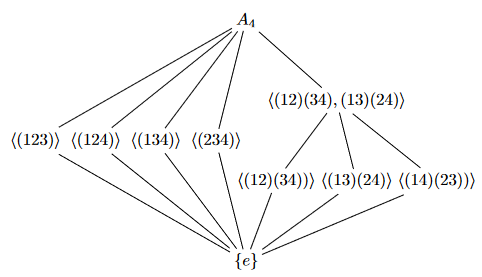
\includegraphics[scale=0.5]{A4.png}
\end{center}

Partition the ten subgroups of $A_4$ into equivalent classes by conjugacy. Then,
pick one subgroup $H$ from each class, find its normalizer $N_{A_4}(H)$, determine the index $[A_4 : N_{A_4}(H)]$, and decide whether or not $H$ is normal.
\begin{proof}

\end{proof}

\item The purpose of the previous part was to serve as a gentle ``warm-up"
for the following. Let $H$ be a subgroup of a finite group $G$, and consider the
following three quantities:
    \begin{enumerate}[(i)]
        \item $[G : H]$, the number of cosets of $H$ in $G$;
        
        \item $|\{gHg^{-1}| g \in G\}|$, the number of subgroups conjugate to $H$;

        \item $[G : N_{G}(H)]$, the number of cosets of the normalizer of $H$ in $G$.
    \end{enumerate}
Two of these are always equal to each other, and one can be different. State and prove the correct equality and the inequality.
\begin{proof}

\end{proof}

\item Consider the action of a $p$-group $G$ (i.e., $|G| = p^n$) on a finite set $X$,
which is just a homomorphism $\phi: G \rar S_X$ to the permutations of $X$. Prove that
$$|X| \equiv |\text{Fix}(\phi)| \ \ (\text{mod } p),$$
where $\text{Fix}(\phi)$ are the fixed points of the action. You may assume that the size
of any orbit divides $|G|$; this is immediate by the orbit-stabilizer theorem.
\begin{proof}

\end{proof}

\item By considering the action of $G$ on $\{gHg^{-1}| g \in G\}$ by conjugation,
and using Part (c), show that the inequality from Part (b) is always strict for
proper subgroups of a $p$-group.
\begin{proof}

\end{proof}
\end{enumerate}












\end{itemize}